% MAEG4060 — Stage 2 Development Report (recreated from PDF text)
\documentclass[11pt,a4paper]{article}

\usepackage[margin=2.5cm]{geometry}
\usepackage[T1]{fontenc}
\usepackage{lmodern}
\usepackage{microtype}
\usepackage{graphicx}
\usepackage[hidelinks]{hyperref}

% Images extracted from 2nd_Report_docs.docx (see ../2nd_Report_docs_images/)
\graphicspath{{../report_images/}}

\title{MAEG4060 Stage 2 Development Report}
\author{%
  \parbox{0.92\linewidth}{\centering
  \textbf{Names \& IDs:}\\[0.35em]
  Guo Tsun Hei (1155186272): 3D Modeling, Texturing, Rigging, and Animation\\
  Yim Fu Chong (1155176974): Programming, Physics Engine, and System Integration}}
\date{}

\begin{document}
\maketitle

\section{Landscape Model}

The landscape will be generated programmatically using a heightmap. The heightmap asset has been finalized.

\begin{figure}[htbp]
  \centering
  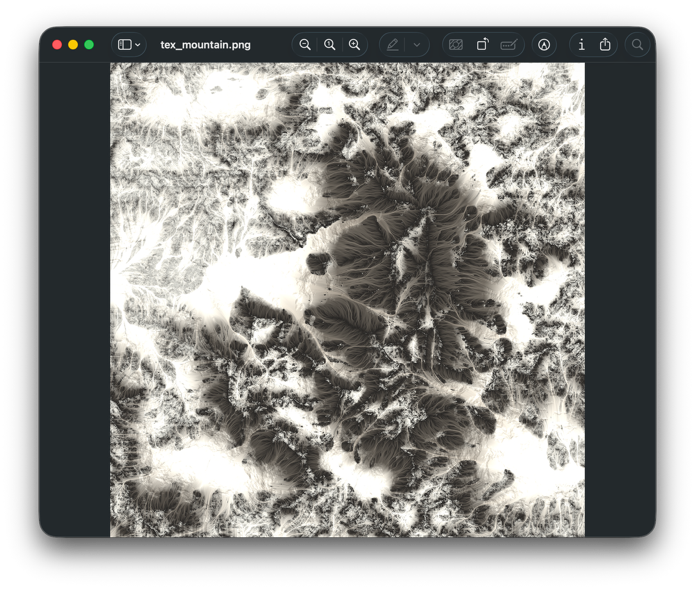
\includegraphics[width=0.48\linewidth]{image1.png}\hfill
  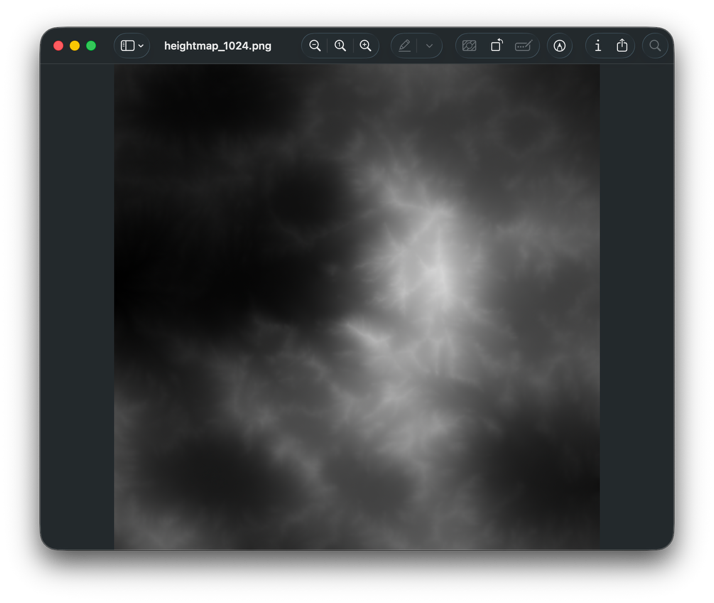
\includegraphics[width=0.48\linewidth]{image2.png}
  \caption{Terrain assets: heightmap and texture (from project documentation).}
\end{figure}

\section{3D Models and Textures}

All required static and controllable models have been acquired, textured, and successfully converted into the DirectX compatible \texttt{.x} format.

\textbf{Files included in submission:}\\[0.25em]
{\ttfamily\small
Assets/models/model\_jeep.x,\allowbreak\ Assets/models/model\_windmill.x,\allowbreak\ Assets/models/model\_crate.x,\allowbreak\ Assets/models/model\_boulder.x}\\
\small\textit{(adjust to match your actual submission bundle.)}

\begin{figure}[htbp]
  \centering
  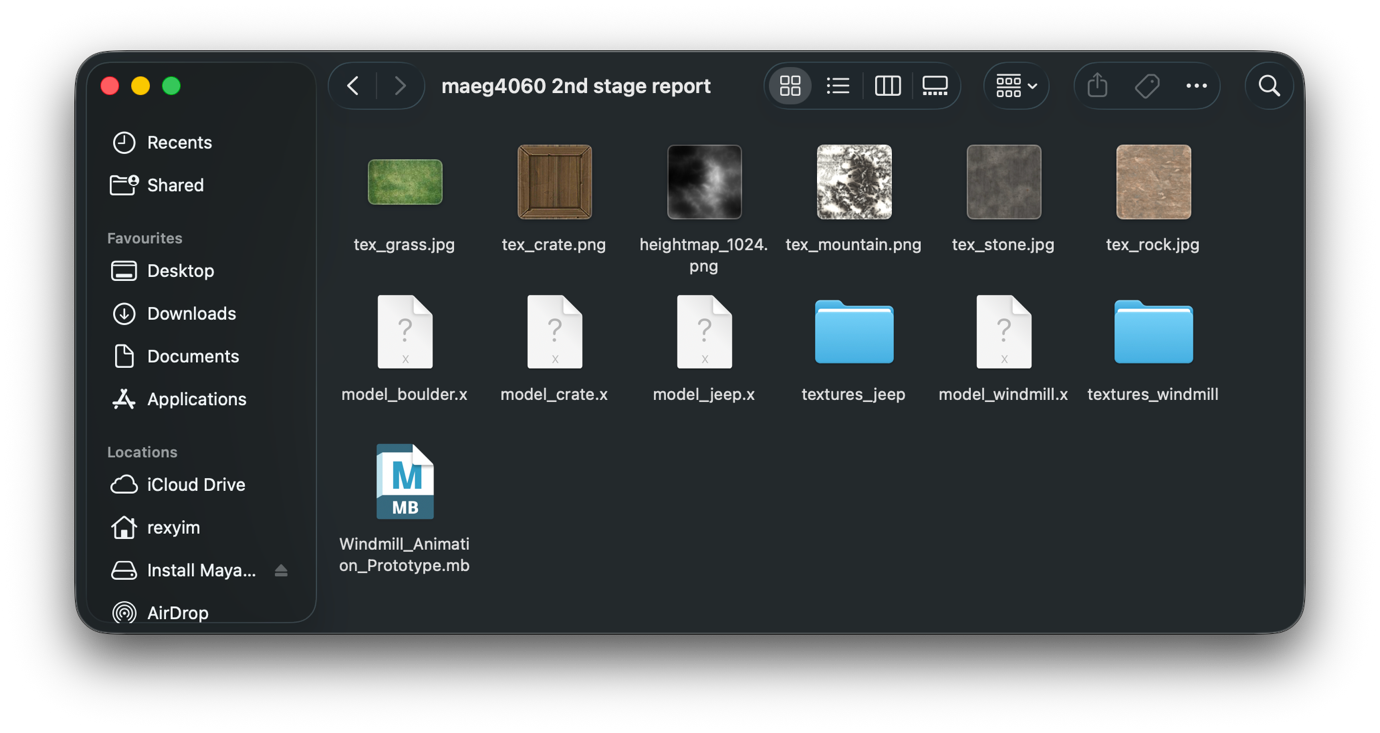
\includegraphics[width=0.32\linewidth]{image3.png}\hfill
  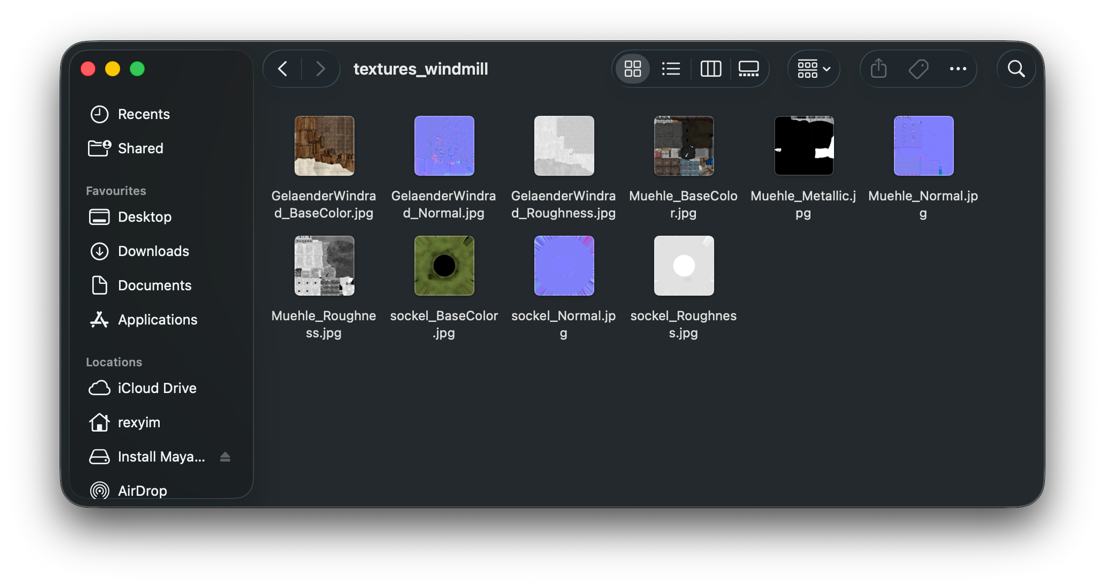
\includegraphics[width=0.32\linewidth]{image4.png}\hfill
  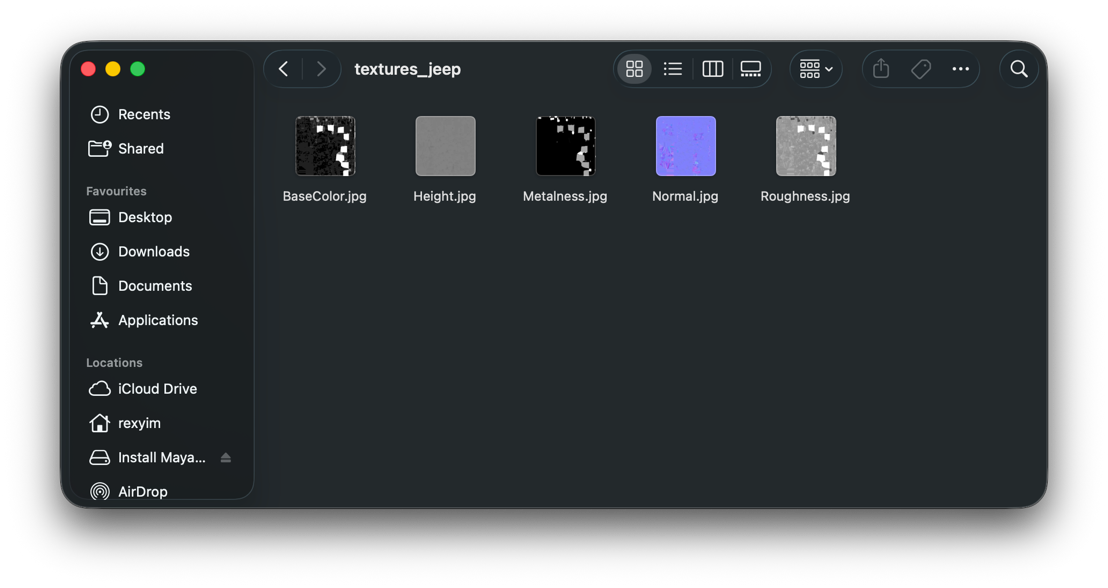
\includegraphics[width=0.32\linewidth]{image5.png}
  \caption{Textured models prepared for \texttt{.x} export and engine integration.}
\end{figure}

\section{Model Animation (Maya)}

To satisfy the animation requirement, the rotational animation for the Windmill was keyframed inside Autodesk Maya. The hierarchical structure allows the engine to parse the animation frames for playback.

\begin{figure}[htbp]
  \centering
  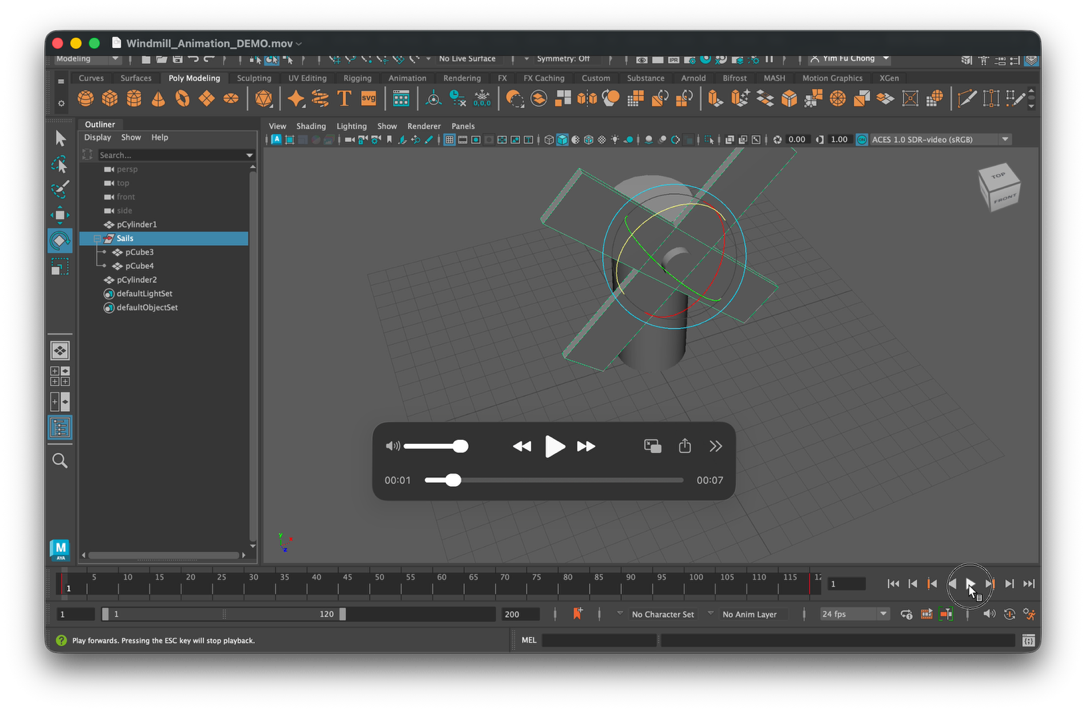
\includegraphics[width=0.92\linewidth]{image6.png}
  \caption{Autodesk Maya: windmill rig and keyframed rotation (timeline visible).}
\end{figure}

\end{document}
